\documentclass[supercite]{HustGraduPaper}
\hypersetup{
colorlinks=true,
linkcolor=black}
\title{浅析居民消费异质性及其对经济增长路径的影响} 
\author{罗浩威} 
\date{\today} 
\school{经济学院} 
\classnum{经济学创新实验班1501} 
\stunum {U201515868} 
\instructor{王健} 
\usepackage{xltxtra}
\usepackage{bm}
\usepackage{natbib}
\begin{document}
    \maketitle
    \statement
    \clearpage 
    \pagenumbering{Roman}
    
    \begin{cnabstract}{异质性消费;经济增长路径;理论分析}
    西方传统的生命周期-持久收入假说对于经济缺乏解释力,因此本文结合异质性消费者的概念在理论上对中国家庭的消费-储蓄行为进行探究,结合北京大学社会科学调查中心的中国家庭追踪调查2012年的横截面数据依据资产结构与特性对隶属于不同类型消费者的家庭进行识别,并在Diamond模型的基础上结合资产结构与流动性分析消费异质性对于经济增长均衡路径的影响,从多方面考察在此框架下不同因素对居民福利的影响。最终综合上述理论与实证,对于中国经济现状提出简要的政策建议。
        
    \end{cnabstract}

    \tableofcontents
    \clearpage
    \pagenumbering{arabic}

    \section{引言}
    中国经济崛起与金融市场、房地产市场的不断开放与改革后,居民财产得以迅速积累,据中国家庭金融调查与研究中心的《中国家庭金融资产配置风险报告2016》所统计,中国家庭净资产年均复合增长率达9.1$\%$,而家庭财产结构及不同组成部分的特性将对消费产生重要的影响。与此同时,在新的全球环境下消费正逐渐代替出口与投资拉动,成为经济增长的新动力。而我国长期以来居民消费水平与人均GDP之比不断下滑,从1996年的47.7$\%$滑落至2011年的35.7$\%$,下滑比例达12$\%$之多。如何协调消费与储蓄、投资的关系,建立扩大消费需求的长效机制,释放中国居民强大的消费潜力成为了问题的关键,对居民消费行为的研究及对消费于经济增长路径所造成影响的分析将具有一定的重要性。
    
    传统的生命周期-持久收入假说(Friedman,1957;Hall,1978)对于分析家庭消费-储蓄决策与宏观经济发展有着较强的指导性,但经济学家通过数据发现现实情况与生命周期-持久收入假说或基于该模型的Buffer-Stock模型(Deaton 1991;Carroll 1997)的预测都有一定出入。例如,无论在宏观或微观层面都可观察到消费支出对于暂时性收入冲击具有较强的敏感性,而生命周期-持久收入中对于暂时性收入冲击不应出现较大的边际消费倾向(MPC,marginal propensity to consume),且现实中我国居民由于资本市场发展尚不完善,投资渠道单一,资产变现时需支付较高的变现成本,这也不符合生命周期-持久收入假说中资产变现、平滑消费0交易成本的设定。对于此一系列现象可尝试打破传统理论中代表性消费者的假定,转而建立模型使资产性质与结构的差异对消费者的消费路径产生影响,即产生异质性消费者。异质性消费者理论最早由Campbell$\&$Mankiw(1989)发展起来,相较于传统模型,异质性消费理论对于经济数据更具解释力(Mankiw,2000),后续实证研究也证明了其合理性(Chyi$\&$Huang,1997;Himarios,2000)。异质性消费者理论的发展对于国家财政政策与货币政策也产生了一定了影响(Gali et al,2005;Morita,2015;Natvik,2012),依据该理论,美国政府多次退税以刺激消费,微观数据可证实居民对于临时性收入冲击具有正的边际消费倾向(Misra$\&$Surico,2014;Johnson et al,2006;Shapir$\&$Slemrod,2003)。除以缺乏流动性资产、缺少信贷渠道来解释异质性消费(Zeldes,1989),也有学者从“有限理性”及信息不完全出发,解释“短视”消费为实际消费路径与最优化消费路径产生偏差的原因(Lettau$\&$Uhlig,1999;Blanchard,1985;Kotlikoff et al,1988)。Kaplan$\&$Violante(2014)开创性地假定居民中存在一部分的HtM消费者(hand-to-mouth consumers),此类消费者在每个支付期中都将可变现使用的资源全部用于消费开支,则可解释即使对于可预期的收入冲击,消费依然与暂时性收入波动呈现较高的相关性。HtM消费者假设目前存在的问题在于前人结合家庭金融调查数据并根据以净资产数额判断异质性消费者的方法发现净资产近乎于零、只得耗尽每期收入用于消费的消费者在人口中占比太小,不足以在数据中显现出上述的效果。已有文献中的异质性消费者理论框架并不注重对家庭资产结构及不同资产流动性与收益加以探究,且对于HtM消费者的判断由于采用净资产作为标准从而遗漏了拥有大量“低流动性,高收益”资产的消费者。本文首先将结合“高流动性,低收益”与“低流动性,高收益”两类资产对家庭进行分类并建立跨期消费决策模型以探究不同类型消费者行为方式的差异及其成因,其次使用北京大学社会科学调查中心的中国家庭追踪调查(China Family Panel Studies,CFPS)2012年的横截面数据和基于前文推导出的分类标准对于中国家庭HtM类消费者占比情况做出初步估量,再次运用资产流动性与资产结构的异质化与Diamond模型相结合以探究经济体系的均衡发展路径及在此框架下经济可能出现的问题,最终对于中国经济现状做出政策建议。

    \section{异质性消费者理论}
    本文将家庭持有资产分为以现金、支票及商业银行存款为代表的“高流动性、低收益”资产和与之相反的以住房资产为代表的“低流动性、高收益”资产两类,资产流动性的高低之分在于资产变现时交易成本的高低。此外,本文将居民按资产配置结构及消费行为特征分为三类,即W-HtM消费者、P-HtM消费者和N-HtM消费者。HtM消费者(hand-to-mouth consumers)指因缺少高流动性资产而无法跨期动态平滑消费的消费者,此类消费者受到流动性约束,只得将当期收入用于消费开支。W-HtM消费者(wealthy hand-to-mouth consumers)和P-HtM消费者(poor hand-to-mouth consumers)同属于HtM消费者,这两类消费者的共同点在于其资产配置结构中同样缺乏高流动性资产,但W-HtM消费者相比P-HtM消费者拥有丰厚的低流动性资产,而P-HtM消费者缺少甚至没有此类资产。N-HtM消费者(non hand-to-mouth consumers)指持有充足高流动性资产从而满足生命周期-持久收入假说可以平滑消费路径的消费者。
    
    根据上述的分类,本文将建立跨期消费决策模型以说明HtM类消费者消费行为的决定因素,v该模型同样可用于确定居民所处的HtM状态。假设模型中的家庭仅生存于$t=0,1,2$三期,且显然,家庭仅在$t=1,2$时进行消费。设定家庭效用函数为
    \begin{equation} 
    v_0=u(c_1)+u(c_2) 
    \end{equation}
    以体现家庭消费时的偏好,$c_t$表示t期的非耐用品消费。假定每一期中的效用函数$u(c_t)$满足$u'>0$,$u''<0$。由于借贷相当于是对高流动性资产的补充,降低家庭在平滑消费时遭遇流动性约束的资产临界值,而效用的主观贴现率主要影响跨期消费的相对价格及消费水平,两者对结论不会产生影响,所以处于简化分析的目的,本文暂不考虑此两种因素。

    假定在期初即$t=0$时,家庭拥有的初始禀赋为$\omega$,可将$\omega$用于$a$、$m_1$两种资产的配置。$a$属于“低流动性,高收益”资产。在$t=2$,家庭要做出消费决策时$a$以资产收益率的形式提供净收益$R$,但在$t=1$,家庭制定消费决策时$a$无法用于平滑当期的消费。$m_1$属于“高流动性,低收益”资产,在$t=1$、$t=2$两期皆可用于家庭的消费,但设定其收益率为$1<R$。假设在进行初期的资产配置后,家庭在$t=1$时获得收入$y_1$,并于此时将$y_1$的一部分用于当期消费,另一部分储蓄为“高流动性,低收益”资产,在$t_2$时家庭获得收入$y_2$并将所持有的全部资产用于消费,即包括$y_2$、$t=1$时储蓄后家庭持有的“高流动性,低收益”资产$m_2$、$t=0$时初始禀赋中“低流动性,高收益”的部分$a$以及家庭所持有资本引致的资本收入。此处$(y_1,y_2)$于$t=0$时已为家庭所知,因此不存在不确定性,则本模型的关键在于分析不同类型消费者在$t=0$时的资产配置决策与$t=1$时的消费-储蓄决策。

    该家庭是HtM消费者或N-HtM消费者取决于$m_2$是否大于零,而该家庭是P-HtM消费者或W-HtM消费者取决于初期禀赋的资产配置中$a$是否大于零。若模型中的家庭为N-HtM消费者,即拥有充足的“高流动性,低收益”资产,在平滑消费时不受到流动性约束,则在$t=1$期消费完后仍可储蓄“高流动性,低收益资产”,可记为$a \geq 0$、$m_2>0$。且由(2.1)式及$u'>0$、$u''<0$可知,如果$c_1 \neq c_2$,假定为$c_1<c_2$,则$t=1$时消费的边际效用$u'$要高于$t=2$期,只需增加$c_1$,即可提高总效用$v_0$,反之亦然,因此对于N-HtM消费者$c_1=c_2$。若模型中的家庭为W-HtM消费者,则应在$t=1$期后拥有数量较多的“低流动性,高收益”资产,但无“高流动性,低收益”资产,可记为$a>0$、$m_2=0$。若模型中的家庭为P-HtM消费者,则在$t=1$期消费后不持有上述的两种资产,可记为$a=0$、$m_2=0$。初期禀赋的资产配置最优化问题可表示为:
    \begin{align*} 
    v_0= & \max_{m_1,a} u(c_1)+u(c_2)\\
    & s.t.\\
    a+m_1= & \omega\\
    c_1+m_2= & y_1+m_1\\
    c_2= & y_2+m_2+Ra\\
    m_1 \geq & 0,a \geq 0 
    \end{align*}
    以上约束条件分别代表了初期禀赋的资产配置问题和$t=1,2$两期时消费面临的预算约束。求解此最优化问题可得关于$a$的一阶条件为
    \begin{equation}
    u'(c_1)[1+\frac{\partial m_2}{\partial a}] \geq u'(c_2)[R+\frac{\partial m_2}{\partial a}]
    \end{equation}
    且$a=0$时左式严格大于右式。导数${\partial m_2}/{\partial a}$反映了$t=0$时“低流动性,高收益”资产持有量对$t=1$时消费-储蓄决策的影响,而该决策同样可等同于对有约束条件下最优化问题的求解,且在$t=1$时$a$与$m_1$的数额已经确定,则该问题可表示为:
    \begin{align*} 
    v_1(a)= & \max_{c_1,m_2} u(c_1)+u(c_2)\\
    & s.t.\\
    c_1+m_2= & y_1+\omega-a\\
    c_1+m_2= & y_1+m_1\\
    c_2= & y_2+m_2+Ra\\
    m_2 \geq & 0
    \end{align*}
    可求解一阶条件为:
    \begin{equation}
    u'(c_1) \geq u'(c_2)
    \end{equation}
    当$m_2=0$时$u'(c_1)>u'(c_2)$成立。(2.3)式可视为$t=1$期消费-储蓄决策的短期欧拉方程。当$m_2=0$时,$a$对$m_2$的数量并无影响,即${\partial m_2}/{\partial a} = 0$,而$m_2>0$时,该家庭属于N-HtM消费者,则可知对该家庭而言有$u'(c_1)=u'(c_2)$,则由上述两个一阶条件结合可得
    \begin{equation}
    u'(c_1) \geq Ru'(c_2)
    \end{equation}
    即长期欧拉方程。对比长短期欧拉方程可发现,因为家庭仅在$t=0$时有储蓄“低流动性,高收益”资产的机会,所以对家庭而言,在$t=0$期时$t=1,2$期消费的相对价格为$R$,而在$t=1$期时,此相对价格减少为1。由短期欧拉方程可得
    \begin{equation}
    m_2=\max \lbrace \frac{y_1+\omega-y_2-(1+R)a}{2},0 \rbrace
    \end{equation}
    即当$y_1+\omega-y_2-(1+R)a \leq 0$时,$m_2=0$,家庭面临流动性约束且可判断此家庭为HtM类消费者。出于简化分析的目的,可仅考虑$m_2=0$的一充分条件$y_2 \geq y_1+\omega$,此充分条件表示,对于某固定数量的初始禀赋$\omega$,当$y_2$在数量上远胜于$y_1$时,即使将全部的初始禀赋储蓄为“高流动性,低收益”资产用于平滑当期消费,$m_2=0$依然成立,即$m_1=\omega,a=0$仍无法满足$t=1$期的消费需求。

    假定效用函数$u$遵循CES(constant elasticity of substitution)函数形式且跨期替代弹性为$\sigma$,则依据长期欧拉方程可求得
    \begin{equation}
    a=\max \lbrace \frac{R^\sigma (y_1+\omega)-y_2}{R+R^\sigma},0 \rbrace
    \end{equation}
    如前文所述,W-HtM消费者满足$a>0$,结合此式即为
    \begin{equation}
    R>(\frac{y_2}{y_1+\omega})^\frac{1}{\sigma}
    \end{equation}
    相反的,对于P-HtM消费者$R$小于等于右式。简要分析此式可发现,跨期替代弹性越高,家庭越倾向于储蓄更多“低流动性,高收益”资产以获得生命周期内整体消费水平的提高,表现出W-HtM消费者的行为特征的可能性更高。同理资产收益率$R$越高也会使家庭更倾向于忍受$t=1$期时可能遭遇流动性约束从而消费不足的情况。但当$y_2/y_1$过高时,由于家庭已确定$t=2$时将获得大笔收入,因此出于平滑消费的目的,家庭储蓄“低流动性,高收入”资产、延缓消费的动机将大大减弱,更有可能表现出P-HtM消费者的行为特征。
    
    \section{我国消费异质性程度估计}
    对于两种HtM消费者,在跨期预算约束问题中有两个节点会存在边际消费倾向MPC较高的情况,即在$t$期中消费尽本期所持有的“高流动性,低收益”资产并无法变现其他资产以平滑消费路径时,或在$t$期结束时消费者已达到信贷限额。定义在获得此次收入之后下次收入之前的时间间隔为一支付期,在模型中,家庭持有的“高流动性,低收益”资产余额将在每期末被估量,而大多数情况下,统计调查仅报告每支付期内的资产平均余额或仅报告家庭接受采访当日的余额情况,则显然这会导致对家庭HtM消费者状态的误判。例如,考虑对跨期消费决策模型进行连续时间的推广,家庭在每支付期期初获得“高流动性,低收益”资产作为收入,期内消费采取连续且速率均匀稳定的方式。则此种情况下,即使HtM类家庭也将显示为拥有一定数额的甚至超越了信贷限额的“高流动性,低收益”资产。

    若统计调查中“高流动性,低收益”资产余额为支付期内的资产余额平均值,记$y_{it}$为家庭$i$在支付期$t$的收入,记$a_{it}$为该家庭在此支付期内持有的“低流动性,高收益”资产的数额,记$m_{it}$为支付期内“高流动性,低收益”资产余额的均值。首先考虑家庭无借贷无“高流动性,低收益”资产储蓄的情况下在支付期$t$开启时获得$y_{it}$并在支付期内以均匀稳定的速率将收入全部用于消费,此时均值满足$m_{it}=y_{it}/2$。因此当家庭满足
    \begin{equation}
    \begin{aligned}
    a_{it} & \leq 0\\
    0 \leq & m_{it} \leq y_{it}/2
    \end{aligned}
    \end{equation}
    时,可识别其为P-HtM消费者,$a_{it}$为负值的情况发生的频率较低,例如家庭住房资产下跌并低于剩余贷款的价值,此类低流动性资产无法带来高收益且无法变现以平滑消费,因此将$a_{it}$小于零的家庭算作P-HtM。而当家庭满足
    \begin{equation}
    \begin{aligned}
    a_{it} & > 0\\
    0 \leq & m_{it} \leq y_{it}/2
    \end{aligned}
    \end{equation}
    时,可识别其为W-HtM消费者。其次对于借贷限额为$-\underline{m_{it}}<0$的家庭,可假定其在支付期开启时借入现金资产$\underline{m_{it}}$并同时获得收入$y_{it}$,并在支付期内将所持有的全部“高流动性,低收益”资产用于消费,则相当于在期内的每一时刻家庭所拥有的“高流动性,低收益”资产相对于无借贷的情况都要减少$\underline{m_{it}}$,即对于P-HtM消费者
    \begin{equation}
    \begin{aligned}
    a_{it} & \leq 0\\
    m_{it} & \leq 0\\
    m_{it} & \leq \frac{y_{it}}{2} - \underline{m_{it}}
    \end{aligned}
    \end{equation}
    对于W-HtM消费者
    \begin{equation}
    \begin{aligned}
    a_{it} & > 0\\
    m_{it} & \leq 0\\
    m_{it} & \leq \frac{y_{it}}{2} - \underline{m_{it}}
    \end{aligned}
    \end{equation}
    以上对于家庭有无借贷两种情况分类并依据“高流动性,低收益”资产平均余额来判别HtM消费者类型的方法仅提供HtM类家庭数量估计值的下限。例如,存在HtM类家庭在支付期开启时持有“高流动性,低收益”资产,但该家庭选择将全部此类资产和收入全部用于当期消费,则该家庭依然会遭遇流动性约束,但在此方法下并不计入HtM类消费者。同样,对于上述模型中借贷限额为$-\underline{m_{it}}<0$的家庭,当$y_{it}$过高时,依然不能按此类方法计入HtM类消费者。

    本文使用北京大学社会科学调查中心的中国家庭追踪调查(China Family Panel Studies,CFPS)2012年的横截面数据。CFPS关注中国居民的各项福利,以及经济活动、教育质量、人口流动等多方面的情况,是一项全国性、跨学科的社会跟踪调查项目。CFPS目标样本规模为16000户,覆盖25个省/市/自治区。CFPS在2008、2009两年在京、沪、粤三地分别开展了初访与追访以进行测试,并于2010年正式开展访问。考虑到统计口径问题和金融资产公允价值计量及相应的可比性问题,本文仅选用并整理2012年的横截面数据作为样本。剔除数据不完整的家庭后剩余9140个样本,且考虑到部分家庭受访时遗漏隐形收入、对收入或财产进行瞒报将导致估计结果的不准确,于是剔除总收入小于等于总支出的家庭,最终得到5812个家庭的数据可用于估量消费异质性的程度。可知人均消费与人均净收入之比计算可得平均消费倾向(average propensity to consume),“高流动性,低收益”资产数额为家庭人均总金融资产除去非房贷的金融负债,“低流动性,高收益”资产数额为家庭净房产、土地资产等。样本主要变量描述性统计如下图
    \begin{generalfig}[htbp]{主要变量的描述性统计(样本容量5812)}{fig:data_1}
    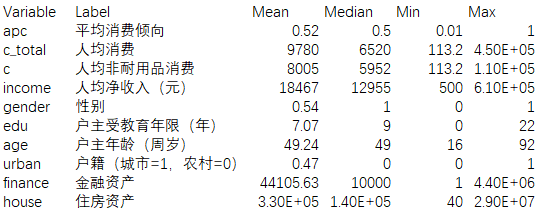
\includegraphics[width=\textwidth]{Figures/data_1.png}
    \end{generalfig}
    
    可知样本中户主男女比接近于1:1,平均年龄为49岁,平均受教育水平为初中阶段,样本平均消费倾向的均值为0.52,城镇户籍与农村户籍之比为47:53,不同家庭贫富差距较大。在对中国家庭HtM类消费者与N-HtM消费者进行占比分析时需要考虑我国具体情况,在我国多数居民收入按月计,因而此处$y_t$为家庭月收入。CFPS提供的收入数据为年收入,假定个月收入均等,则将年收入包括年终奖在内均摊至12个月得月收入。并且由于我国家庭消费信贷普及率很低且相较于欧美国家储蓄率较高,则在区分P-HtM消费者与W-HtM消费者时以$a_{it}=0$为标准将造成较大偏差,因此本文设定标准为$a_{it}=y_t$以进行分类判断。且在现实中,中国家庭不仅会在春节、中秋节等传统节日消费支出突然增大,在“双十一”等电子商务促销的节点中国家庭同样会出现突击性消费的情况,因此匀速消费的假定略有不妥,出于稳健性的考虑,本文将对判断标准予以进一步的调整。以$0.25y_t$、$0.5y_t$、$0.75y_t$作为不同的判别标准以进行估量。由统计结果可知,无论判别标准如何变动,在HtM类家庭内部,W-HtM类型家庭占比要远高于P-HtM类型的家庭。仅观察以模型中原始假定的$0.5y_t$为判断标准的结果,HtM类型家庭中有93.49$\%$的家庭为W-HtM类型,P-HtM类型仅占6.51$\%$。中国家庭不同类型消费者的占比情况可与世界其他国家进行对比研究。
    \begin{generalfig}[htbp]{HtM类家庭与N-HtM家庭占比分析(样本容量5812)}{fig:data_2}
    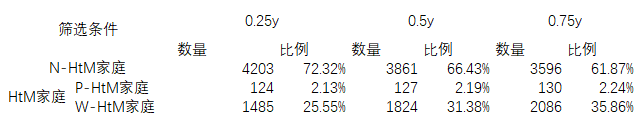
\includegraphics[width=\textwidth]{Figures/data_2.png}
    \end{generalfig}
    
    Kaplan$\&$Violante(2014)利用跨国微观数据估量发现美国、加拿大与德国HtM类型家庭占比约为30$\%$,此数值与本文估量的中国家庭的情况相近,但澳大利亚、法国、西班牙、意大利此数值略低于我国,约为20$\%$。各国在P-HtM类型家庭与W-HtM类型家庭的相对数量上存在较大差异,澳大利亚、法国、西班牙此数值与我国接近,意大利P-HtM类型家庭在HtM类型中占比略高于我国,为$7.4\%$,其余国家皆在$10\%$以上。

    \section{消费异质性对经济增长路径的影响}
    基于Diamond模型构建包含“高流动性,低收益”及“低流动性,高收益”两种资产的经济增长模型,借此浅析家庭资产结构与异质性消费对于经济增长均衡路径的影响。在此模型中假定存在人口组成的更替,每期内都存在新生人口进入模型与死亡人口离开模型。为简化分析起见,假定时间为离散而非连续的,并且一个独立个体在模型中仅存活两期,即生命周期的上下半期,对应时间节点为$t=0,1,2$。设有数量为$L_{t}$的个体在$t$期出生且人口增长率为$n$,则$L_{t}=(1+n)L_{t-1}$。既然个体仅存活两期则出现于同一期内的个体,部分处于其生命周期上半期,人数为$L_{t}$,部分处于其生命周期下半期,人数为$L_{t-1}=L_{t}/(1+n)$。处于生命周期上半期的每个个体可供给一单位劳动并在该期内做出消费-储蓄决策,在生命的下半周期,个体随着年龄的增长不在劳动,将生命周期上半期的储蓄及资本收入全部用于下半期的消费。可简单理解为,劳动收入中用于当期收入的部分为“高流动性,低收益”资产而用于储蓄至下半周期并产生资本收入的部分为“低流动性,高收益”资产。分别将生命上半周期及下半周期的消费记为$C_{1,t}$、$C_{2,t+1}$,记出生于$t$的个体整个生命周期内的效用为$U_{t}$,且可假定效用函数遵循CRRA(constant-relative-risk-aversion)函数形式以便于求得经济增长的均衡路径。此处由于生命周期有限,因此无需考虑因模型参数设置不当而导致生命周期效用发散的情况。设$\rho$个体的主观贴现率,相对风险回避系数为常数$\theta$,则该效用函数具体可设为两期消费的效用之和
    \begin{equation}
    \begin{aligned}
    U_{t}=\frac{C_{1,t}^{1-\theta}-1}{1-\theta}+&\frac{1}{1+\rho}\frac{C_{2,t+1}^{1-\theta}-1}{1-\theta}\\
    \theta>0,\qquad & \rho>-1
    \end{aligned}
    \end{equation}
    因为下半个生命周期消费的效用贴现后应为正值,个体主观贴现率$\rho$必须大于-1。当$\rho$大于零时,生命周期下半期消费效用的权重$0<\frac{1}{1+\rho}<1$,即个体将更倾向于重视生命周期上半期的效用情况,当$\rho$小于零大于-1时,则相反。假定模型中有多家完全相同的企业制造产出,每一家企业的生产函数皆为$Y_{t}=F(K_{t},A_{t}L_{t})$,生产函数为规模报酬不变,即对任意大于等于零的常数$c$都有$F(cK,cAL)=cF(K,AL)$,同时生产函数满足稻田条件。可设每单位有效劳动$AL$对应资本量为$k$,对应产出则为$f(k)=F(k,1)=F(K,AL)/AL$。全要素生产率或配合生产的技术知识$A$保持外生性增长率$g$,即$A_{t}=(1+g)A_{t-1}$。由于劳动供给市场与产品市场为完全竞争,则生产要素资本与劳动都获得其边际产量作为报酬,所有厂商利润为零,则参与生产的资本所获得的实际利率为$r_t=f'(k_t)$,每单位有效劳动所获报酬为$w_t=f(k_t)-k_tf'(k_t)$,对个体而言,收入将分配用于消费或储蓄为资本获得报酬,既然已知消费为$C_{1,t}$,则储蓄的数额为$w_tA_t-C_{1,t}$。假设初期资产数量$K_0$均匀分布于所有处于生命周期下半期的个体,此时处于生命周期上半期的个体提供劳动以制造产出,伴随着人口的更替与每期储蓄与消费的分配,模型将不断演进下去。对于$t$期出生的个体,$t+1$期消费可表示为
    \begin{equation}
    C_{2,t+1}=(1+r_{t+1})(w_tA_t-C_{1,t})
    \end{equation}
    将等式两边同除以$1+r_{t+1}$后整理可得
    \begin{equation}
    C_{1,t}+\frac{1}{1+r_{t+1}}C_{2,t+1}=A_{t}w_{t}
    \end{equation}
    则个体生命周期内消费的现值与劳动所获收入的现值相等,此式可视为生命周期内消费的预算约束。因此求解个体消费-储蓄决策即求解最优化问题
    \begin{equation}
    \begin{aligned}
    \max U_{t}=\frac{C_{1,t}^{1-\theta}-1}{1-\theta}+&\frac{1}{1+\rho}\frac{C_{2,t+1}^{1-\theta}-1}{1-\theta}\\
    s.&t.\\
    C_{1,t}+\frac{1}{1+r_{t+1}}C_{2,t+1}&=A_{t}w_{t}
    \end{aligned}
    \end{equation}
    假设个体略微减少生命周期上半期消费$C_{1,t}$用于储蓄,减少的数额记为$\Delta C$,则相当于减少“高流动性,低收益”资产的持有,增持“低流动性,高收益”资产,$C_{2,t+1}$将因此而增加$(1+r_{t+1})\Delta$,两期的消费依旧满足预算约束。可知如个体处于最优化效用的消费水平,则趋近于零的$\Delta C$不会改变整体的效用水平,即减少$C_{1,t}$带来的效用损失将恰好为$C_{2,t+1}$增加所带来的效用增益所弥补。如非如此,个体将重新调整两期消费的数额以实现整体效用水平的上升,即此时个体的效用水平并未达到预算约束下的最优化,与前提矛盾。求导可知,对于生命周期内整体效用水平$U_{t}$,$C_{1,t}$与$C_{2,t+1}$的边际效用分别为$C_{1,t}^{-\theta}$与$[1/(1+\rho)]C_{2,t+1}^{-\theta}$。$\Delta C$趋近于零时,效用的改变量为边际效用与$\Delta C$的乘积,则最优化要求
    \begin{equation}
    C_{1,t}^{-\theta}\Delta C=\frac{1}{1+\rho}C_{2,t+1}^{-\theta}\Delta C
    \end{equation}
    整理可得
    \begin{equation}
    \frac{C_{2,t+1}^\theta}{C_{1,t}^\theta}=\frac{1+r_{t+1}}{1+\rho}
    \end{equation}
    \begin{equation}
    \frac{C_{2,t+1}}{C_{1,t}}=\frac{1+r_{t+1}}{1+\rho}^{1/\theta}
    \end{equation}
    当资本的实际回报率或实际利率大于主观折现率时,两期而言消费将增加,反之,则下半期消费较上半期减少。$\theta$则决定了个体消费情况对$r$与$\rho$大小变化的反应程度。将此欧拉方程代入预算约束可得
    \begin{equation}
    C_{1,t}+\frac{(1+r_{t+1})^{(1-\theta)/\theta}}{(1+\rho)^{1/\theta}}C_{1,t}=A_tw_t
    \end{equation}
    整理可得
    \begin{equation}
    C_{1,t}=\frac{(1+\rho)^{1/\theta}}{(1+\rho)^{1/\theta}+(1+r_{t+1})^{(1-\theta)/\theta}}A_tw_t
    \end{equation}
    由于$\rho$与$\theta$皆为常数,则可知生命周期上半期的消费占劳动收入的比例由实际利率决定,可将储蓄率表示为$s(r_{t+1})$,则有$s(r_{t+1})=1-C_{1,t}/A_tw_t$,具体有
    \begin{equation}
    \begin{aligned}
    s(r)=\frac{(1+r)^{(1-\theta)/\theta}}{(1+\rho)^{1/\theta}+(1+r)^{(1-\theta)/\theta}}\\
    C_{1,t}=[1-s(r_{t+1})]A_tw_t
    \end{aligned}
    \end{equation}
    $s(r)$对于$(1+r)^{(1-\theta)/\theta}$是增函数,可将$(1+r)^{(1-\theta)/\theta}$对实际利率$r$求导可得$[(1-\theta)/\theta](1+r)^{(1-2\theta)/\theta}$,则当$\theta$小于1时,此式对于$r$递增,同样也储蓄率$s$对于$r$递增,相反,当$\theta$大于1时,$s$对于$r$递减。从经济意义上讲,实际利率$r$增加对消费同时具有替代效应和收入效应,当$r$增加时,放弃储蓄在生命周期上半期及时消费的成本变高了。可视为“低流动性,高收益”资产的变现成本更高,因此个体会倾向于在上半期减少消费增加储蓄,而与此同时,同样数额的储蓄将获得更多的资本收入,个体不用大量储蓄收入即可在生命周期下半期充分地享受消费,处于平滑消费的目的,个体会倾向于在上半期增加消费而减少储蓄。当$\theta$较低时,个体对于上下半期消费的替代弹性更高,则此时替代效应起主要作用,而$\theta$较高时,消费的替代弹性较低,个体更愿意在两期内享受相近的消费水平,则收入效应起主要作用。当$\theta$恰好为1时,效用函数采取对数形式,且有$s(r)=1/(2+\rho)$,储蓄率不再和$r$有关。

    根据模型的设定,在$t+1$期资本存量为$t$期内处于生命周期上半期的个体所储蓄,即可记为
    \begin{equation}
    K_{t+1}=s(r_{t+1})L_tA_tw_t
    \end{equation}
    将等式两边同除以$t+1$期有效劳动$L_{t+1}A_{t+1}$则有
    \begin{equation}
    k_{t+1}=\frac{1}{(1+n)(1+g)}s(r_{t+1})w_t
    \end{equation}
    将前文中所推导出的公式代入此式可得出$k_{t+1}$作为因变量$k_t$作为自变量的方程,可表示此模型中每一单位有效劳动所获得的资本存量$k$的发展路径
    \begin{equation}
    k_{t+1}=\frac{1}{(1+n)(1+g)}s(f'(k_{t+1}))[f(k_t)-k_tf'(k_t)]
    \end{equation}
    如果存在资产存量值$k_t$处于均衡发展路径之上则应满足$k_t=k_{t+1}$,当资产存量达到此值时就不会再变动。如未对资本存量发展路径函数做特殊假定则很难讨论是否存在均衡发展路径,开始于某一数额的资本存量的经济体所达到的稳态值是否唯一,$k$收敛于该值的速率如何等较为复杂的问题。因此出于分析的需要,暂时简单假定$\theta=1$,如前文所述,此时储蓄率$s=1/(2+\rho)$。且假定生产函数满足Cobb-Douglas形式,$f(k)=k^\alpha$则$f'(k)=\alpha k^{\alpha-1}$。此时$k$的发展路径简化为
    \begin{equation}
    k_{t+1}=\frac{1}{(1+n)(1+g)}\frac{1}{2+\rho}(1-\alpha)k_{t}^\alpha
    \end{equation}
    令$k_{t+1}=k_t=k*$为稳态下的资本存量值,显然当$k*=0$时上式成立,但此种情况由于已假定初始资本存量$K_0$严格大于零而被排除,则由函数形态可判断仅剩一点$k*$可满足
    \begin{equation}
    k*=\frac{1}{(1+n)(1+g)}\frac{1}{2+\rho}(1-\alpha)k*^\alpha
    \end{equation}
    解得
    \begin{equation}
    k*=[\frac{1-\alpha}{(1+n)(1+g)(2+\rho)}]^{1/(1-\alpha)}
    \end{equation}
    且由于生产函数已知,得到每单位有效劳动的产出
    \begin{equation}
    y*=k*^\alpha=[\frac{1-\alpha}{(1+n)(1+g)(2+\rho)}]^{\alpha/(1-\alpha)}
    \end{equation}
    经济中暂时存在不同的$k_t$值也将向$k*$收敛,例如设初始值$k_0$大于$k*$,因为由函数形态可知在$k$值超越稳态之后,$k_{t+1}$将小于$k_t$,又因为资本存量的发展路径为增函数,则有$k*<k_1<k_0$,并且$k_2$、$k_3$等等后续的资本存量值都将处于上一期资本存量值与均衡发展路径上的值$k*$之间,在长期中资本存量值$k_t$将不断趋近于$k*$,直至最终达至稳态不再变动。初始值$k_0$小于$k*$情况下的分析与此类似不再赘述。可发现,在均衡增长路径上,储蓄率为常数,每个个体劳动产出增长速率恒定为$A$的增长率$g$且资本-产出比保持不变。若探究经济趋近于均衡发展路径的具体情况,可设$k'_{t+1}(k*)=\lambda$,即将资本存量发展路径在$k*$处的导数记为$\lambda$。根据线性化,在均衡发展路径周围有$k_{t+1}-k*\backsimeq\lambda(k_t-k*)$,进一步推演即得到$k_t-k*\backsimeq\lambda^t(k_0-k*)$。可见趋近于均衡发展路径的情况与$\lambda$密切相关。可求解此导数值
    \begin{equation}
    \begin{aligned}
    \lambda &=\alpha\frac{1-\alpha}{(1+n)(1+g)(2+\rho)}k*^{\alpha-1}\\
    &=\alpha\frac{1-\alpha}{(1+n)(1+g)(2+\rho)}[\frac{1-\alpha}{(1+n)(1+g)(2+\rho)}]^{\alpha-1/(1-\alpha)}
    &=\alpha
    \end{aligned}
    \end{equation}
    可见$\lambda$为Cobb-Douglas生产函数中的系数$\alpha$,系数$\alpha$在0到1之间,则经济将平滑地趋近于均衡发展路径。若非限定为效用函数采取对数形式且生产函数采取Cobb-Douglas函数形式,可分情况讨论$\lambda$,位于0至1之间的情况无需多言,当其在-1到0之间时,资本存量值将围绕均衡发展路径表现出逐渐减弱的上下波动并最终收敛,如其大于1则最终资本存量值将趋于正无限而不会收敛于均衡发展路径,如其小于-1则资本存量值将围绕$k*$上下剧烈波动且无法收敛。    
    
    可考察不同的冲击或修正对此简易模型中经济均衡发展路径的影响。例如,最初经济处于平衡发展路径之上,当主观贴现率$\rho$突然降低时,由$s=1/(2+\rho)$可知储蓄率将上升,新达成的稳态资本存量值$k*_{NEW}$将高于原值$k*_{OLD}$,但达成新的稳态后其增长速率并无变化。又例如,在此模型中加入政府部门以考察财政政策对均衡发展路径的影响。记$t$期每单位有效劳动对应的政府购买数额为$G_t$并假定政府购买完全以来自处于生命周期上半期个体的缴税为支撑,此时每单位有效劳动获得的收入将减少为$(1-\alpha)k_t^\alpha-G_t$,资本存量的发展路径也变为
    \begin{equation}
    k_{t+1}=\frac{1}{(1+n)(1+g)}\frac{1}{2+\rho}[(1-\alpha)k_{t}^\alpha-G_t]
    \end{equation}
    则对于每一个$k_t$而言,下一期的资本存量$k_{t+1}$相对于无政府部门的情况都减少了,则资本存量发展路线的曲线将下移,可推断最终收敛于的稳态值,即该曲线与$45^{\circ}$对角线的交点$k*_{NEW}$将低于$k*_{OLD}$,此时实际利率也将更高。

    此模型指出经济可能存在资本过度积累的问题,无法达成Pareto最优,即所谓动态无效率问题。在此模型中,出生于不同时期的个体将在整个生命周期内享有不同水平的效用,则暂无衡量社会福利的有效方法,将不同年代个体的效用赋以不同权重进行加总毫无意义,因为权重的大小更多是出于随意的安排而非具有某种理论依据。

    在假定对数形式效用函数与Cobb-Douglas形式生产函数的基础上进一步假定$A$的外生增长率$g=0$。可求解得
    \begin{equation}
    k*=[\frac{1}{1+n}\frac{1}{2+\rho}(1-\alpha)]^{1/(1-\alpha)}
    \end{equation}
    则在均衡发展路径上资本的边际产出为
    \begin{equation}
    f'(k*)=\alpha k*^{\alpha-1}=\frac{\alpha}{1-\alpha}(1+n)(2+\rho)
    \end{equation}
    黄金法则(golden-rule)下的资本存量定义为在此$k_{GR}$下每单位有效劳动对应的总消费可达到最大值。总消费数额为每单位有效劳动对应的产出$f(k)$减去使每期资本存量维持不变的储蓄额也即投资额$nk$,对$c_{GR}(k_{GR})$求导并令之等于0可求得$f'(k_{GR})=n$。本文中$f'(k*)$与$n$的大小暂无法确定。当$\alpha$过于小时,$f'(k*)<f'(k_{GR})=n$,由于资本的边际产出(marginal product)递减,则可知$k*>k_{GR}$,可见此模型下均衡发展路径并不能使个人效用达到最优化。

    设想如在$t_0$时社会共同决定在达到资本存量处于均衡发展路径之上后,社会个体共同改变消费-储蓄决策以期下一期资本存量将达到黄金法则下的水平$k_{GR}$并长久地维持下去。则$t_0$时个体消费数额为$f(k*)+(k*-k_{GR})-nk_{GR}$,在此之后每期的消费数额就变为$f(k_{GR}-nk_{GR})$。如此可知采取此项政策后每一期每单位有效劳动对应的消费都要高于之前资本存量稳定于$k*$的情况。并且社会可在此基础上进行转移支付以使每代居民的效用都得到增加,可知每个个体都对应$(1+n)$个下一代个体,若$(1+n)$位下一代个体每人支付对应的同一位上一代个体一单位劳动收入,则上一代个体消费增加$(1+n)$个单位,此政策不断延续下去,当处于生命周期上半期的个体转移支付劳动收入后将在生命周期下半期通过下一代的转移支付而得到补偿。此政策即为Pareto改进,可证实资本存量为$k*$时并未达到Pareto有效。

    原模型框架下产生资本过度积累、动态无效率是因为如果个体希望进入生命周期下半期时能够维持一定的消费水平,他唯一的方式就是将更多的劳动收入储蓄为“低流动性,高收益”资产,即使此时资本收益率相较之下并不算“高”。因此由于此模型中资产缺乏跨期的流动性,个体无法实现消费的跨期动态优化并被迫进行预防性储蓄而面对流动性约束。当模型在无限期内执行转移支付时,个体消费不再受制于单一的渠道和存在下跌风险的资本收益率,可实现Pareto改进,释放消费潜力。
    
    \section{结论与政策建议}
    为进一步释放我国居民的消费潜力,应继续大力促进我国资本市场的发展与完善,削弱国有银行为主体的金融垄断势力,在监管金融风险的同时鼓励金融创新,开发出更多期限不同收益率不同风险特质不同的金融产品以满足居民对于金融多样性的需要,提高金融服务的可得性,开展普惠金融,让大众共享中国经济高速发展带来的红利。

    在政府购买与征税会降低均衡增长路径的资本存量的前提下,应提高政府支出的效益,避免低水平重复建设,大力推进供给侧改革以拓展内需促进消费,实现产业升级。

    完善租房市场,早日实现“租售同权”,对于户籍权益、教育医疗等资源的分配尽量平等,降低由于房地产市场不确定性导致的预防性储蓄与流动性约束。

    建立运转高效的福利制度,在失业救济、养老、医疗保障方面加大投入以减少不确定性以解决消费者的后顾之忧,扩大当期消费。

    \bibliographystyle{elsarticle-num}
    \bibliography{mybib}
    
    \begin{thankpage}
    四年前怀抱着对经济学的好奇,我考入经济学创新实验班1501。大学匆匆的光阴里,我有幸得到了经济学院学识渊博、谆谆善诱的老师们的悉心指导,或许多年后脑海中曾经鲜活的经济学思想的阐释只剩下不过只言片语,但四年来体会到的来自前辈师长的温情终身难忘,在这里尤其感谢指导我毕业论文写作的王健老师,在我迷茫困顿时与我长谈的张卫东老师、张玉英老师、邱慧芳老师和易鸣老师。路漫漫其修远兮,吾将上下而求索,对经济学的探索于我才刚刚开始,在新的路途上,我将常常怀想经济学院老师们的勤奋与严谨。现在我将暂时与母校作别,此番拜离,情深意长,一语难表。
    \end{thankpage}


\end{document}







